\let\negmedspace\undefined
\let\negthickspace\undefined
\documentclass[journal]{IEEEtran}
\usepackage[a5paper, margin=10mm, onecolumn]{geometry}
%\usepackage{lmodern} % Ensure lmodern is loaded for pdflatex
\usepackage{tfrupee} % Include tfrupee package

\setlength{\headheight}{1cm} % Set the height of the header box
\setlength{\headsep}{0mm}     % Set the distance between the header box and the top of the text

\usepackage{gvv-book}
\usepackage{gvv}
\usepackage{cite}
\usepackage{amsmath,amssymb,amsfonts,amsthm}
\usepackage{algorithmic}
\usepackage{graphicx}
\usepackage{textcomp}
\usepackage{xcolor}
\usepackage{txfonts}
\usepackage{listings}
\usepackage{enumitem}
\usepackage{mathtools}
\usepackage{gensymb}
\usepackage{comment}
\usepackage[breaklinks=true]{hyperref}
\usepackage{tkz-euclide} 
\usepackage{listings}
% \usepackage{gvv}                                        
\def\inputGnumericTable{}                                 
\usepackage[latin1]{inputenc}                                
\usepackage{color}                                            
\usepackage{array}                                            
\usepackage{longtable}                                       
\usepackage{calc}                                             
\usepackage{multirow}                                         
\usepackage{hhline}                                           
\usepackage{ifthen}                                           
\usepackage{lscape}
\begin{document}

\bibliographystyle{IEEEtran}
\vspace{3cm}

\title{2.3.6}
\author{EE25BTECH11003 - Adharvan Kshathriya Bommagani}
% \maketitle
% \newpage
% \bigskip
{\let\newpage\relax\maketitle}

\renewcommand{\thefigure}{\theenumi}
\renewcommand{\thetable}{\theenumi}
\setlength{\intextsep}{10pt} % Space between text and floats
\textbf{Question}:\\
Find the magnitude of each of the vectors $\vec{a}$ and $\vec{b}$ , having the same magnitude
such that the angle between them is 60\degree and their scalar product is $\frac{9}{2}$ .
  
\bigskip

\textbf{Solution}:\\

We are given two vectors $\vec{a}$ and $\vec{b}$ with the same magnitude, and the angle between them is $60^\degree$. Also, their scalar product is given as:
\begin{align}
\vec{a}^T \vec{b} = 2.
\end{align}

\bigskip





Let the common magnitude of the vectors be $r$, i.e., $\|\vec{a}\| = \|\vec{b}\| = r$.
Let the magnitudes of the two vectors be equal:
\begin{align}
\|\mathbf{a}\| = \|\mathbf{b}\| = r.
\end{align}

The cosine of the angle between the two vectors is given by:
\begin{align}
\cos\theta = \frac{\mathbf{a}^T \mathbf{b}}{\|\mathbf{a}\|\,\|\mathbf{b}\|}.
\end{align}

Substituting $\|\mathbf{a}\| = \|\mathbf{b}\| = r$, this simplifies to:
\begin{align}
\cos\theta = \frac{\mathbf{a}^T \mathbf{b}}{r^2}.
\end{align}

Since the angle between the vectors is $60^\circ$, we have $\cos 60^\circ = \frac{1}{2}$.  
The scalar product is given as $\mathbf{a}^T \mathbf{b} = \frac{9}{2}$. Substituting these values:
\begin{align}
\frac{1}{2} = \frac{\frac{9}{2}}{r^2}.
\end{align}


Multiply through by $2r^2$:
\begin{align}
r^2 = 9.
\end{align}

Taking the positive root (since magnitude cannot be negative):
\begin{align}
r = +3.
\end{align}

\begin{align}
r = 3
\end{align}



Therefore the magnitude of the vectors $\vec{a}$ and $\vec{b}$ is 3 each.
\newpage
\textbf{Two vectors with magnitude 3 and angle $\mathbf{60\degree}$ between them}
\begin{figure}[H]
    \centering
    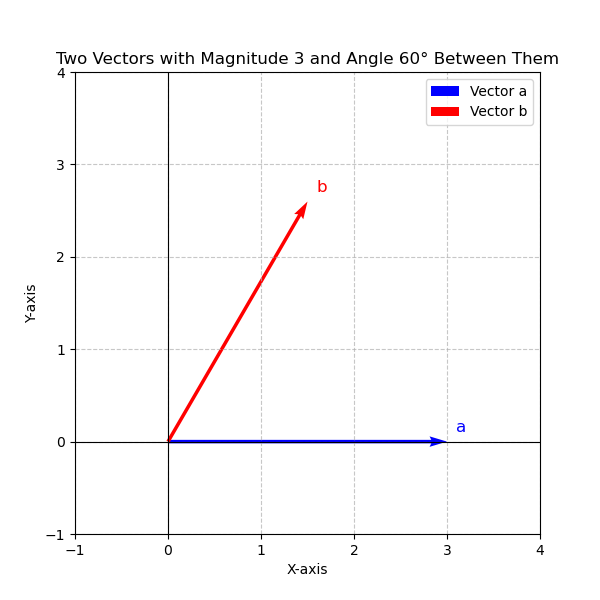
\includegraphics[width=1.1\columnwidth]{figs/fig1.png}
    \caption{Figure for 2.3.6}
    \label{fig1}
\end{figure}

\end{document}
























